% Hai slide phần ALS và Cholesky, để người ghép slide \input vào file beamer chung.
% Số liệu đo trên MovieLens-1M, tập val.
\begin{frame}{ALS: mỗi bước là hàng nghìn hệ Ridge}
  \textbf{Ý tưởng:} cố định $Q$ thì mỗi $p_u$ là nghiệm của một hệ Ridge (Ch.3):
  \[
    (Q_u^\top Q_u + \lambda I)\, p_u = Q_u^\top r_u
  \]
  \begin{itemize}
    \item $Q_u$ chỉ gồm phim user $u$ đã đánh giá, lấy nhanh từ CSR (Ch.2).
    \item $\lambda > 0$ làm ma trận xác định dương, nên giải được bằng Cholesky tự cài (Ch.2).
    \item Mỗi bước cho nghiệm đúng, nên hàm mục tiêu không tăng và không cần learning rate.
    \item $\lambda$ giảm số điều kiện lớn nhất từ $2\,476$ ($\lambda = 0{,}01$) xuống $6{,}2$ ($\lambda = 10$).
  \end{itemize}
\end{frame}

\begin{frame}{ALS: kết quả trên MovieLens-1M}
  \centering
  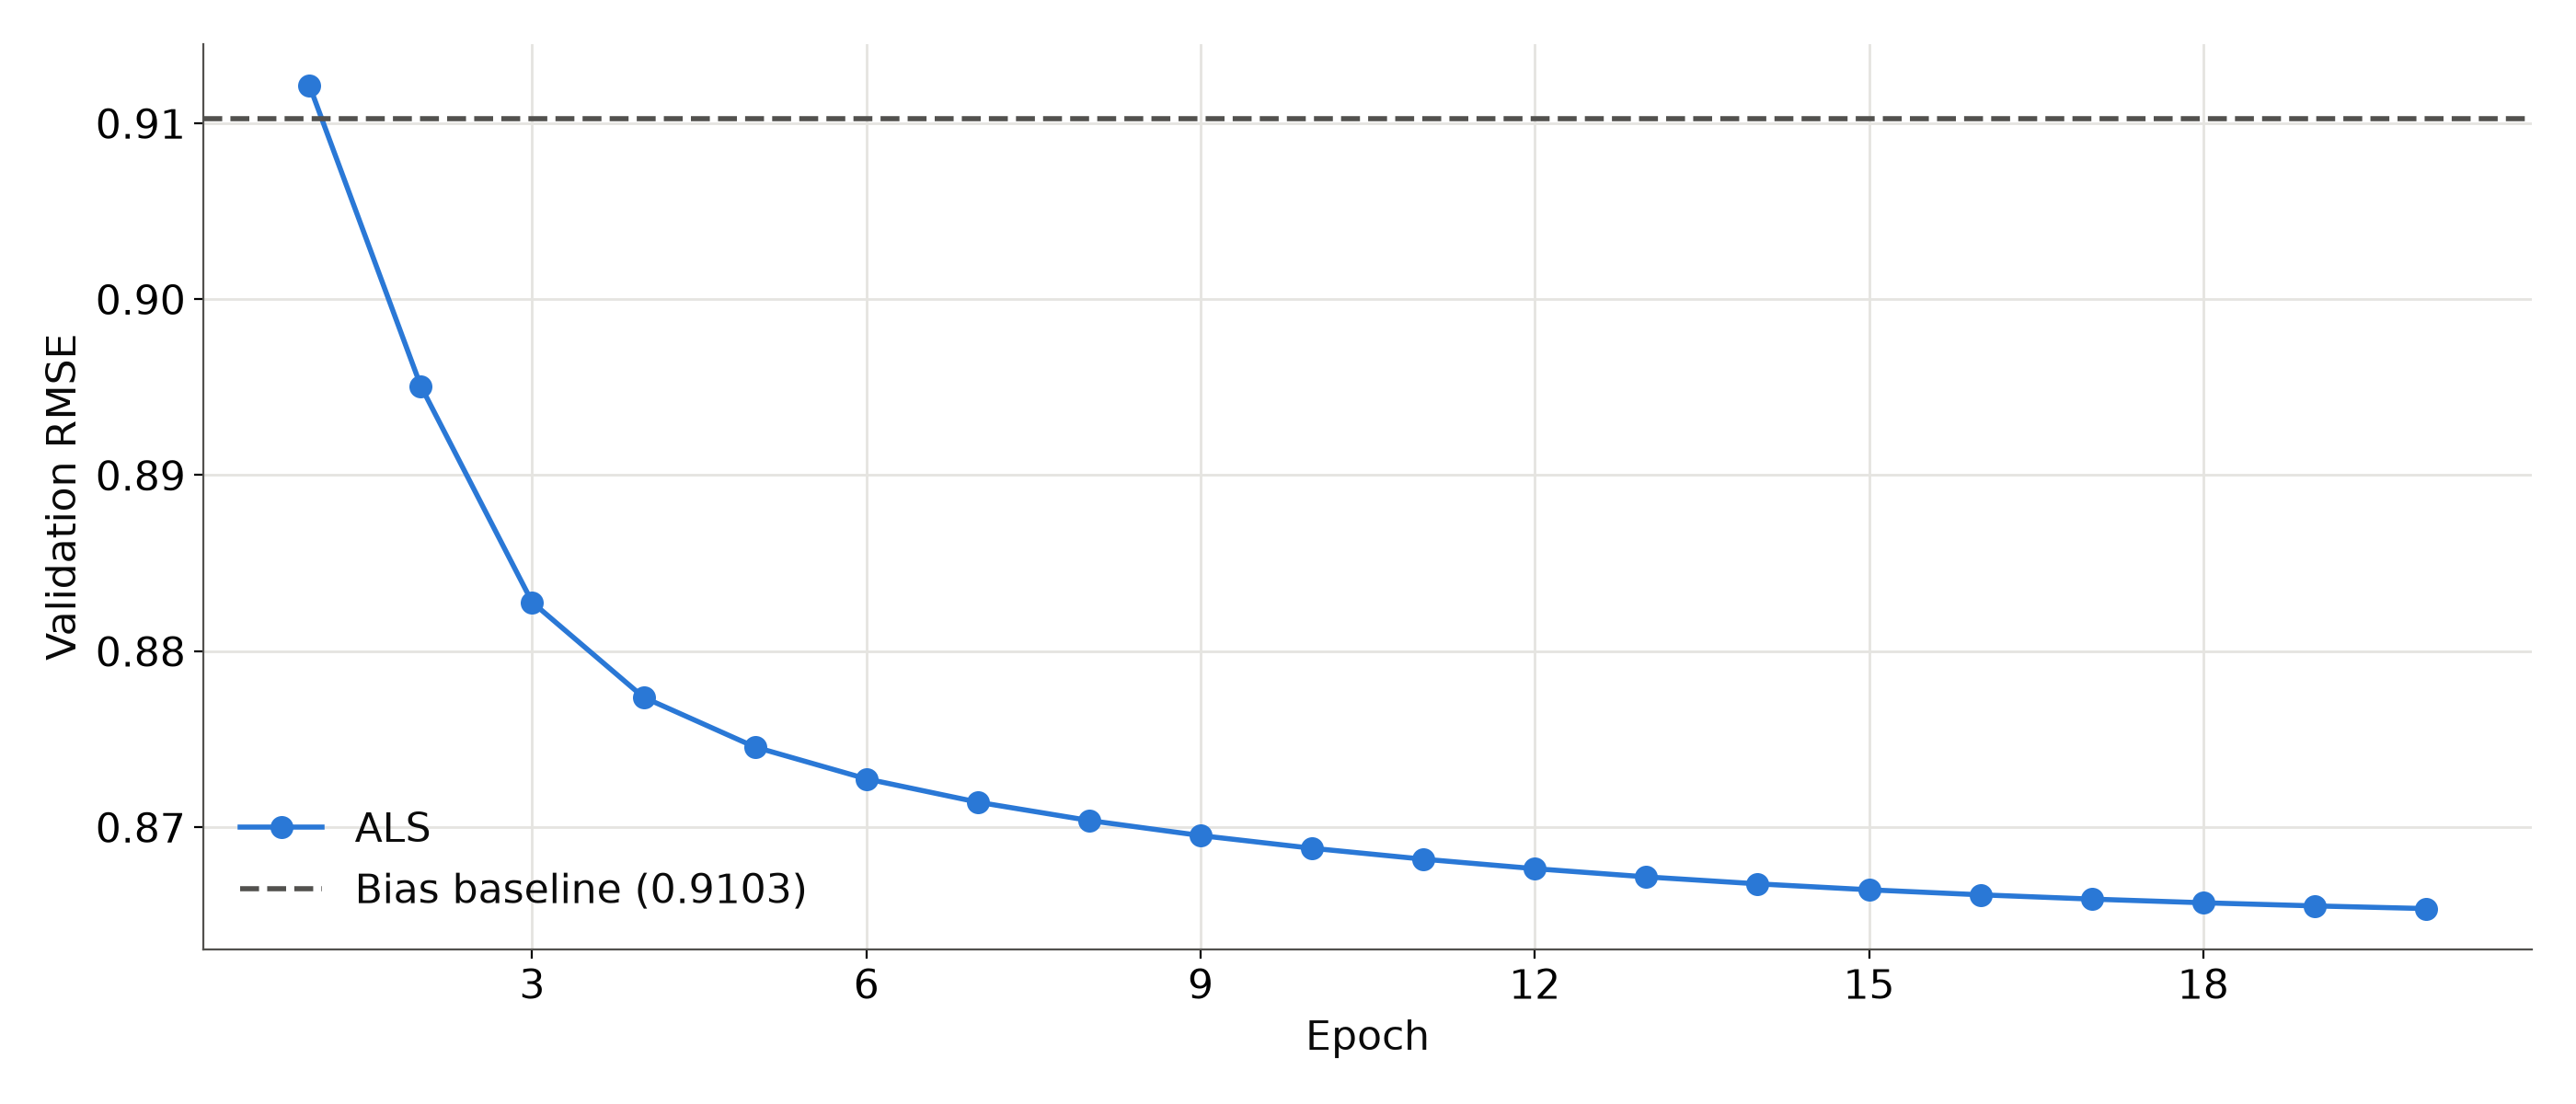
\includegraphics[width=0.85\linewidth]{figures/als_val_rmse_by_epoch.png}
  \begin{itemize}
    \item RMSE val: baseline $0{,}9103$, ALS $0{,}8654$ ($k = 20$, $\lambda = 10$, 20 vòng).
    \item Khoảng $0{,}06$ giây mỗi vòng cho $9\,746$ hệ; dựng $Q_u^\top Q_u$ chiếm phần lớn chi phí, không phải Cholesky.
  \end{itemize}
\end{frame}
